\hypertarget{sfusd}{%
\chapter{The Stanford-SFUSD Partnership: Development of Data-Sharing Structures and Processes}\label{sfusd}}

\printchapterauthor{%
\begin{authorlist}
  Moonhawk Kim (University of California, Berkeley)  \\
  Jim Shen (J-PAL, Massachusetts Institute of Technology)  \\
  Laura Wentworth (California Education Partners)  \\
  Norma Ming (San Francisco Unified School District)  \\
  Michelle Reininger (University of Colorado at Boulder)  \\
  Eric Bettinger (Stanford University)  \\
\end{authorlist}}\authorfootnote{Kim, Moonhawk, Jim Shen, Laura Wentworth, Norma Ming, Michelle Reininger, and Eric Bettinger}{Moonhawk Kim, Jim Shen, Laura Wentworth, Norma Ming, Michelle Reininger, and Eric Bettinger}{sfusd}
\authortoc{Moonhawk Kim, Jim Shen, Laura Wentworth, Norma Ming, Michelle Reininger, Eric Bettinger}
\hrulefill

\hypertarget{summary-5}{%
\section{Summary}\label{summary-5}}

Research-practice partnerships\index{Research-practice partnerships} (RPPs) have a growing reputation for making important connections between the worlds of research and practice in education \citep{farley-ripple2018, farrell2019}. These partnerships are long-term, mutualistic, and strategic relationships between researchers and practitioners in education: the product is research that is both related to practical challenges and generalizable to the broader field \citep{coburn2013, coburn2016}. An essential component of some of these partnerships is the data management and data sharing needed for operationalizing research, yet there is little documentation for how to develop and maintain the data infrastructure to support these partnerships.

To improve the field's understanding of the data infrastructure needed for RPPs, this chapter describes the data infrastructure within the partnership between Stanford University Graduate School of Education (Stanford GSE) and San Francisco Unified School District (SFUSD). The partnership was started in 2009 with SFUSD administrative data being shared on a project-by-project basis.\footnote{See \citet{wentworth2016} for a description of the Partnership's origins} In 2010, given the number of requests for administrative data by Stanford faculty and researchers to be used in research studies with SFUSD, the Stanford-SFUSD Partnership\index{Stanford-SFUSD Partnership} developed an approach to warehousing regular extracts of SFUSD administrative data within a data warehouse\index{data warehouse} at Stanford University. SFUSD administrative data housed at Stanford University captures data on over 55,000 students, over 3,500 PreK--12 teachers, and a total of almost 10,000 staff from the academic year 2000/2001 to the present. Since 2011, when the data warehouse was started, the number of Stanford research projects with SFUSD requesting data from the CEPA Data Manager has tripled from three projects to nine projects in 2018.

This chapter describes the development of this data infrastructure to meet that demand within the Stanford-SFUSD Partnership from its infancy in 2009 to its present state in 2020. The chapter starts by giving the motivation and background as well as cases of data use in research. Then the authors describe SFUSD leaders' ways of conceptualizing the different uses of data as well as capacities and personnel to prepare and supply these data to the Stanford-SFUSD Partnership and other researchers in general. The chapter addresses the legal frameworks guiding the decisions related to the design of infrastructure and agreements, and it explores the case of the Stanford-SFUSD Partnership data infrastructure through the lens of the five safes framework. Finally, the authors summarize some lessons learned that are mentioned throughout the chapter, which could be helpful for the field more broadly and especially for research-practice partnerships that analyze administrative data.

The authors represent current and former members of the Partnership who worked to launch, maintain, or revise the necessary structures and agreements to support the data preparation and exchange. They include Michelle Reininger, the former Executive Director of the Stanford Center for Education Policy Analysis\index{Center for Education Policy Analysis} (CEPA) and research faculty at Stanford GSE, who is now at the University of Colorado; Laura Wentworth, the Director of Research Practice Partnerships at California Education Partners, who continues to direct the Stanford-SFUSD Partnership; current and former administrators in SFUSD who helped improve the agreements and district-side data infrastructure within SFUSD, including Norma Ming, SFUSD's Supervisor of Research and Evaluation in SFUSD's Research, Planning, and Assessment (RPA) division, and Moonhawk Kim, formerly the Supervisor of Analytics in SFUSD's RPA division and now at UC Berkeley; as well as other current and former members at Stanford who helped operationalize the data infrastructure, including Jim Shen, who formerly managed the CEPA data warehouse and is now at J-PAL, and Eric Bettinger, one of the faculty whose research team has accessed and used the data from the warehouse and who is now the faculty director of CEPA where the data are housed at Stanford.

\hypertarget{introduction-6}{%
\section{Introduction}\label{introduction-6}}

\hypertarget{motivation-and-background-4}{%
\subsection{Motivation and Background}\label{motivation-and-background-4}}

This chapter describes the development, design, and use of the data infrastructure for the Stanford-SFUSD Partnership\index{Stanford-SFUSD Partnership}. Established in 2009, the Stanford-SFUSD Partnership supports an average of 25 to 30 active projects at any given time, many of which require administrative data as part of the research. The Partnership maintains a data warehouse\index{data warehouse} at Stanford University that includes data from the academic year 2000/2001---ten years prior to the start of the arrangement---to the present on information related to SFUSD's over 55,000 students across 133 schools and nearly 10,000 staff. The CEPA data warehouse includes information about SFUSD student demographics, school attendance, special programs (e.g., English learner services, Special Education, or after-school programming), academic outcomes (e.g., grades, standardized test scores), behavioral outcomes and interventions (e.g., attendance, office referral), and key milestones (e.g., graduations). These data have been used in projects examining a range of topics such as ethnic studies courses \citep{dee2017}, human capital \citep{dizon-ross2019}, and large-scale school reforms \citep{sun2017}. The partnership started when a number of Stanford GSE faculty were working on projects with SFUSD, and a local funder supporting these research projects asked the SFUSD and Stanford leaders whether they found their work together useful enough to create a more formal partnership that could provide coordination of the different relationships. The funder offered to hire a Partnership director\index{Partnership director} to work with Stanford faculty and SFUSD administrators to support the two organizations when working on research together in hopes of producing mutually beneficial outcomes: generalizable research.

From the outset, the partnership was designed to encourage two institutions---Stanford University GSE and SFUSD---to work together differently, thereby changing some of the status quo practices within each institution and in their collaborations. These included establishing some new processes and agreements for governing the data infrastructure. This started with creating a data warehousing agreement and data use agreement\index{data use agreement} (DUA) template and evolved to include an annual meeting where SFUSD and Stanford leaders convene to discuss data use and research with the goal of calibrating and aligning their efforts.

The processes for governing the data infrastructure evolved over time in response to needs. In the beginning of the partnership, Stanford researchers and the SFUSD research department administrators felt challenged by the volume of data exchanges and the time and resources needed to prepare those data extracts. Also, it took time to develop the DUAs for each project, which had to be reviewed individually by the Stanford and SFUSD legal departments. While SFUSD worked with many researchers, the Stanford-based research projects constituted a significant share of all requests for administrative data from SFUSD. This high volume of requests for administrative data led to an agreement to warehouse SFUSD administrative data at Stanford.

In 2011, the Partnership director worked with the SFUSD research department, Stanford GSE Dean's office, and the leadership of CEPA\index{CEPA} to streamline the agreements needed for data use and access to address the challenges with data exchange. To do this the two institutions' legal departments created a standardized DUA template, which Stanford researchers could easily fill out when submitting data requests to SFUSD. With such a template, the Stanford and SFUSD legal teams would not need to review every project's DUA. An even larger commitment to this partnership came when both SFUSD and Stanford established an umbrella warehousing agreement between Stanford University GSE, CEPA, and SFUSD to house SFUSD data and distribute the necessary data for their research projects to all Stanford researchers with an approved DUA. The warehouse would require personnel and management beyond hiring a Partnership director. This undertaking was key in moving the Stanford-SFUSD Partnership from a federation of projects to an actual partnership.

\hypertarget{data-use-examples-4}{%
\subsection{Data Use Examples}\label{data-use-examples-4}}

Here three cases of research supported through the Stanford-SFUSD Partnership's data infrastructure are described.\footnote{Please note that not all of the journal articles are cited from this research to maintain anonymity of the school district in some specific studies.} This infrastructure has enabled descriptive as well as quasi-experimental and experimental research. Two cases analyze only secondary administrative data collected by SFUSD: the first used descriptive statistics and regression modeling and the second used the method of implementing a quasi-experimental design. The third case collected primary survey data in combination with analyzing secondary administrative data. These cases were selected for a number of reasons. First, these cases represent Stanford researchers and SFUSD leaders who have been working together on lines of inquiry for a substantial amount of time. Second, the research has been influential in SFUSD leaders' decision-making as well as at the state and national levels. Third, these cases showcase some of the statistical methods that the authors thought would be of interest to the audience for this Handbook.

\hypertarget{study-of-english-learner-programs}{%
\subsubsection*{Study of English Learner Programs}\label{study-of-english-learner-programs}}
\addcontentsline{toc}{subsubsection}{Study of English Learner Programs}

This first case describes an example of research using descriptive statistics and regression modeling using de-identified administrative data. To better serve English learners\index{English learners}, SFUSD leaders had adopted four different types of language programs, which provide English language development as well as instruction in another target language. Yet SFUSD leaders lacked reliable local evidence comparing the effectiveness of their bilingual and English-only language programs for English learners. To address this, SFUSD Special Assistant to the Superintendent Christina Wong and Chief of Research, Planning, and Assessment Ritu Khanna partnered with Stanford GSE Professor Sean F. Reardon, a sociologist, to examine the impact of SFUSD's programs on English learners' education outcomes. Reardon and his team worked with SFUSD research department staff to validate and organize the variables in the data across SFUSD's language pathways. With the help of the Strategic Education Research Partnership and the Stanford-SFUSD Partnership director, Khanna, Reardon, Wong, and their teams met about every other month to examine descriptive data reports and preliminary results, to address questions by the researchers, and explore interpretations of the data by the district leaders. The research suggested that over time, English learner students in dual-language programs using both English and their native language developed English and academic skills faster than those immersed in English-only instruction. In addition to producing eight articles published in peer-reviewed academic journals and other types of policy and practice publications, the research helped SFUSD leaders to evaluate and ultimately justify continued implementation and support for their bilingual programs. These findings have been presented at the state level in California and at U.S. conferences, helping to change California's policies in support of bilingual education.

\hypertarget{evaluating-the-impact-of-a-course-in-ethnic-studies}{%
\subsubsection*{Evaluating the Impact of a Course in Ethnic Studies}\label{evaluating-the-impact-of-a-course-in-ethnic-studies}}
\addcontentsline{toc}{subsubsection}{Evaluating the Impact of a Course in Ethnic Studies}

This second case describes an example of research applying a quasi-experimental design to analyze administrative data from the data warehouse\index{data warehouse}. The SFUSD school board adopted a policy to support an ethnic studies\index{ethnic studies} course in their high schools in hopes that the course would help reduce absenteeism and narrow opportunity gaps, in addition to influencing other outcomes like high school dropout rates, truancy, and graduation. A set of SFUSD high schools was selected to pilot the course, and Assistant Superintendent of High Schools Bill Sanderson was in charge of overseeing the pilot and reporting back to the school board on the outcomes. Through the Stanford-SFUSD Partnership\index{Stanford-SFUSD Partnership}, Bill Sanderson collaborated with Stanford GSE Professor Thomas Dee, an economist, to evaluate the ethnic studies course pilot using SFUSD administrative data from the CEPA data warehouse. Applying a regression discontinuity design, Professor Dee's research suggested that the ethnic studies courses in SFUSD's pilot program improved students' GPA and attendance significantly compared to similar students not enrolled in the course \citep{dee2017}. Along with other information presented to the school board, this research helped motivate the board to pass resolution 1410-28A4, ``Institutionalizing Ethnic Studies into the San Francisco Unified School District'' \citep{sanfranciscounifiedschooldistrict2014} to offer an ethnic studies course at all SFUSD high schools. This research has been cited by other school districts \citep{cuevas2019} and states \citep{ragland2017} to justify policies that support ethnic studies courses, including California policymakers as they consider requiring ethnic studies courses across all California high schools.

\hypertarget{evaluating-changes-to-human-capital-policies}{%
\subsubsection*{Evaluating Changes to Human Capital Policies}\label{evaluating-changes-to-human-capital-policies}}
\addcontentsline{toc}{subsubsection}{Evaluating Changes to Human Capital Policies}

This third case describes an example of research combining primary survey data about teachers' perspectives on conditions influencing turnover and retention with secondary SFUSD administrative data from the warehouse. In 2009, San Francisco voters passed the Quality Teacher and Education Act\index{Quality Teacher and Education Act} (QTEA), which supported a parcel tax providing additional funding for teacher salaries in SFUSD among other things \citep{hough2009}. Since that time, SFUSD's Human Resources department has been tasked with implementing the teacher salary increases and teacher bonuses meant to support teachers working in hard-to-staff positions and schools. SFUSD Chief of Human Resources, Daniel Menezes, has continued a relationship with Professor Susanna Loeb, then at Stanford but now at Brown University. Loeb and her research team launched an evaluation of the effects of the increases in SFUSD teacher salaries in 2009, finding some positive influences on teacher recruitment, but less impact on teacher retention \citep{hough2013}. In partnership with SFUSD, Loeb started surveying all SFUSD teachers, principals, and assistant principals in 2009, and even with her transition to Brown University in 2017, has continued the partnership. Since then, Loeb and her colleagues have conducted multiple studies using the teacher and administrator survey data and SFUSD administrative data on students and teachers \citep{dizon-ross2019}. Loeb and her colleagues used quasi-experimental designs to evaluate the effects of the QTEA and other pertinent human capital policies in SFUSD \citep{sun2017}. Chief Menezes and many other leaders have referenced Loeb's research when justifying key human capital decisions. For example, in 2019, San Francisco Mayor London Breed wanted to put city funding towards a research-backed practice, and cited Loeb's research as a rationale for providing increased stipends to teachers working in hard-to-staff schools in San Francisco \citep{waxmann2019}. What has been particularly valuable about this arrangement is having an external research team analyze the teacher survey data in conjunction with other teacher characteristics and outcomes in the administrative data, thus preserving the confidentiality of individual teachers' survey responses.

\hypertarget{making-data-usable-for-research-3}{%
\section{Making Data Usable for Research}\label{making-data-usable-for-research-3}}

A robust data infrastructure must be established for research-practice partnerships to reliably produce studies such as those discussed above. Prior to sharing data for research, both SFUSD and Stanford needed to prepare and process the data. This section describes frameworks to guide data management, SFUSD's and Stanford's approaches for processing the administrative data and building a data infrastructure, and finally, the processes for exchanging the data.

\hypertarget{framework-for-converting-operational-data-to-analytical-data-for-research}{%
\subsection{Framework for Converting Operational Data to Analytical Data for Research}\label{framework-for-converting-operational-data-to-analytical-data-for-research}}

In school districts, as in other large organizations, data serve multiple purposes. While Solberg et al.~\citeyearpar{solberg1997} distinguish between using data for accountability\index{accountability}, improvement\index{improvement}, and research, the authors of this chapter add service provision\index{service provision} and evaluation\index{evaluation} as two additional purposes \citep{sanfranciscounifiedschooldistrict2019}. Whereas \emph{research} is expected to be generalizable, \emph{evaluation} may sometimes be narrowly focused on a local initiative. \emph{Improvement} may draw from both research and evaluation, but it prioritizes informing the local implementers rather than external audiences. \emph{Service provision} is inherently local, using data for such activities as enrolling students, transferring credits, or determining program eligibility. \emph{Accountability} summarizes local data to report to the public, funders, or others in the broader community. These purposes may be mapped on to the distinction between enumerative studies\index{enumerative studies}, which describe the current state, and analytical studies\index{analytical studies}, which draw inferences to apply to a future state \citep{deming1953, provost2011}. Service provision and accountability rely on enumerative studies about the current state, while research and evaluation constitute analytical studies that may generalize more broadly. Improvement may qualify under either category depending on the distance of transfer.

These distinctions are important because the types of activities require different data and their interpretations of data are varied (illustrated in Figure \ref{fig:sfusdfigure1}). Operational data\index{Operational data} describe the current state at a specific point in time and undergo frequent updating to accurately reflect changing conditions, while analytical data\index{analytical data} must capture consistent and comparable snapshots of the operational data. Staff rely on operational data in real time to provide services and to report out accountability metrics at specified times of year. For example, students may switch into and out of an ethnic studies course, shift from one section to another, or even change schools while maintaining enrollment in ethnic studies. Operational data need to reflect these changes in real time for schools and teachers to accurately maintain records of students' course-taking and provide service. By contrast, analytical data need to freeze the operational data to facilitate replicable and reproducible research and evaluation studies. Students who took ethnic studies in a school year need to be defined by some criteria, such as students who were enrolled by a specific date and those who remained enrolled for a minimum percentage of the school year.

\begin{figure}
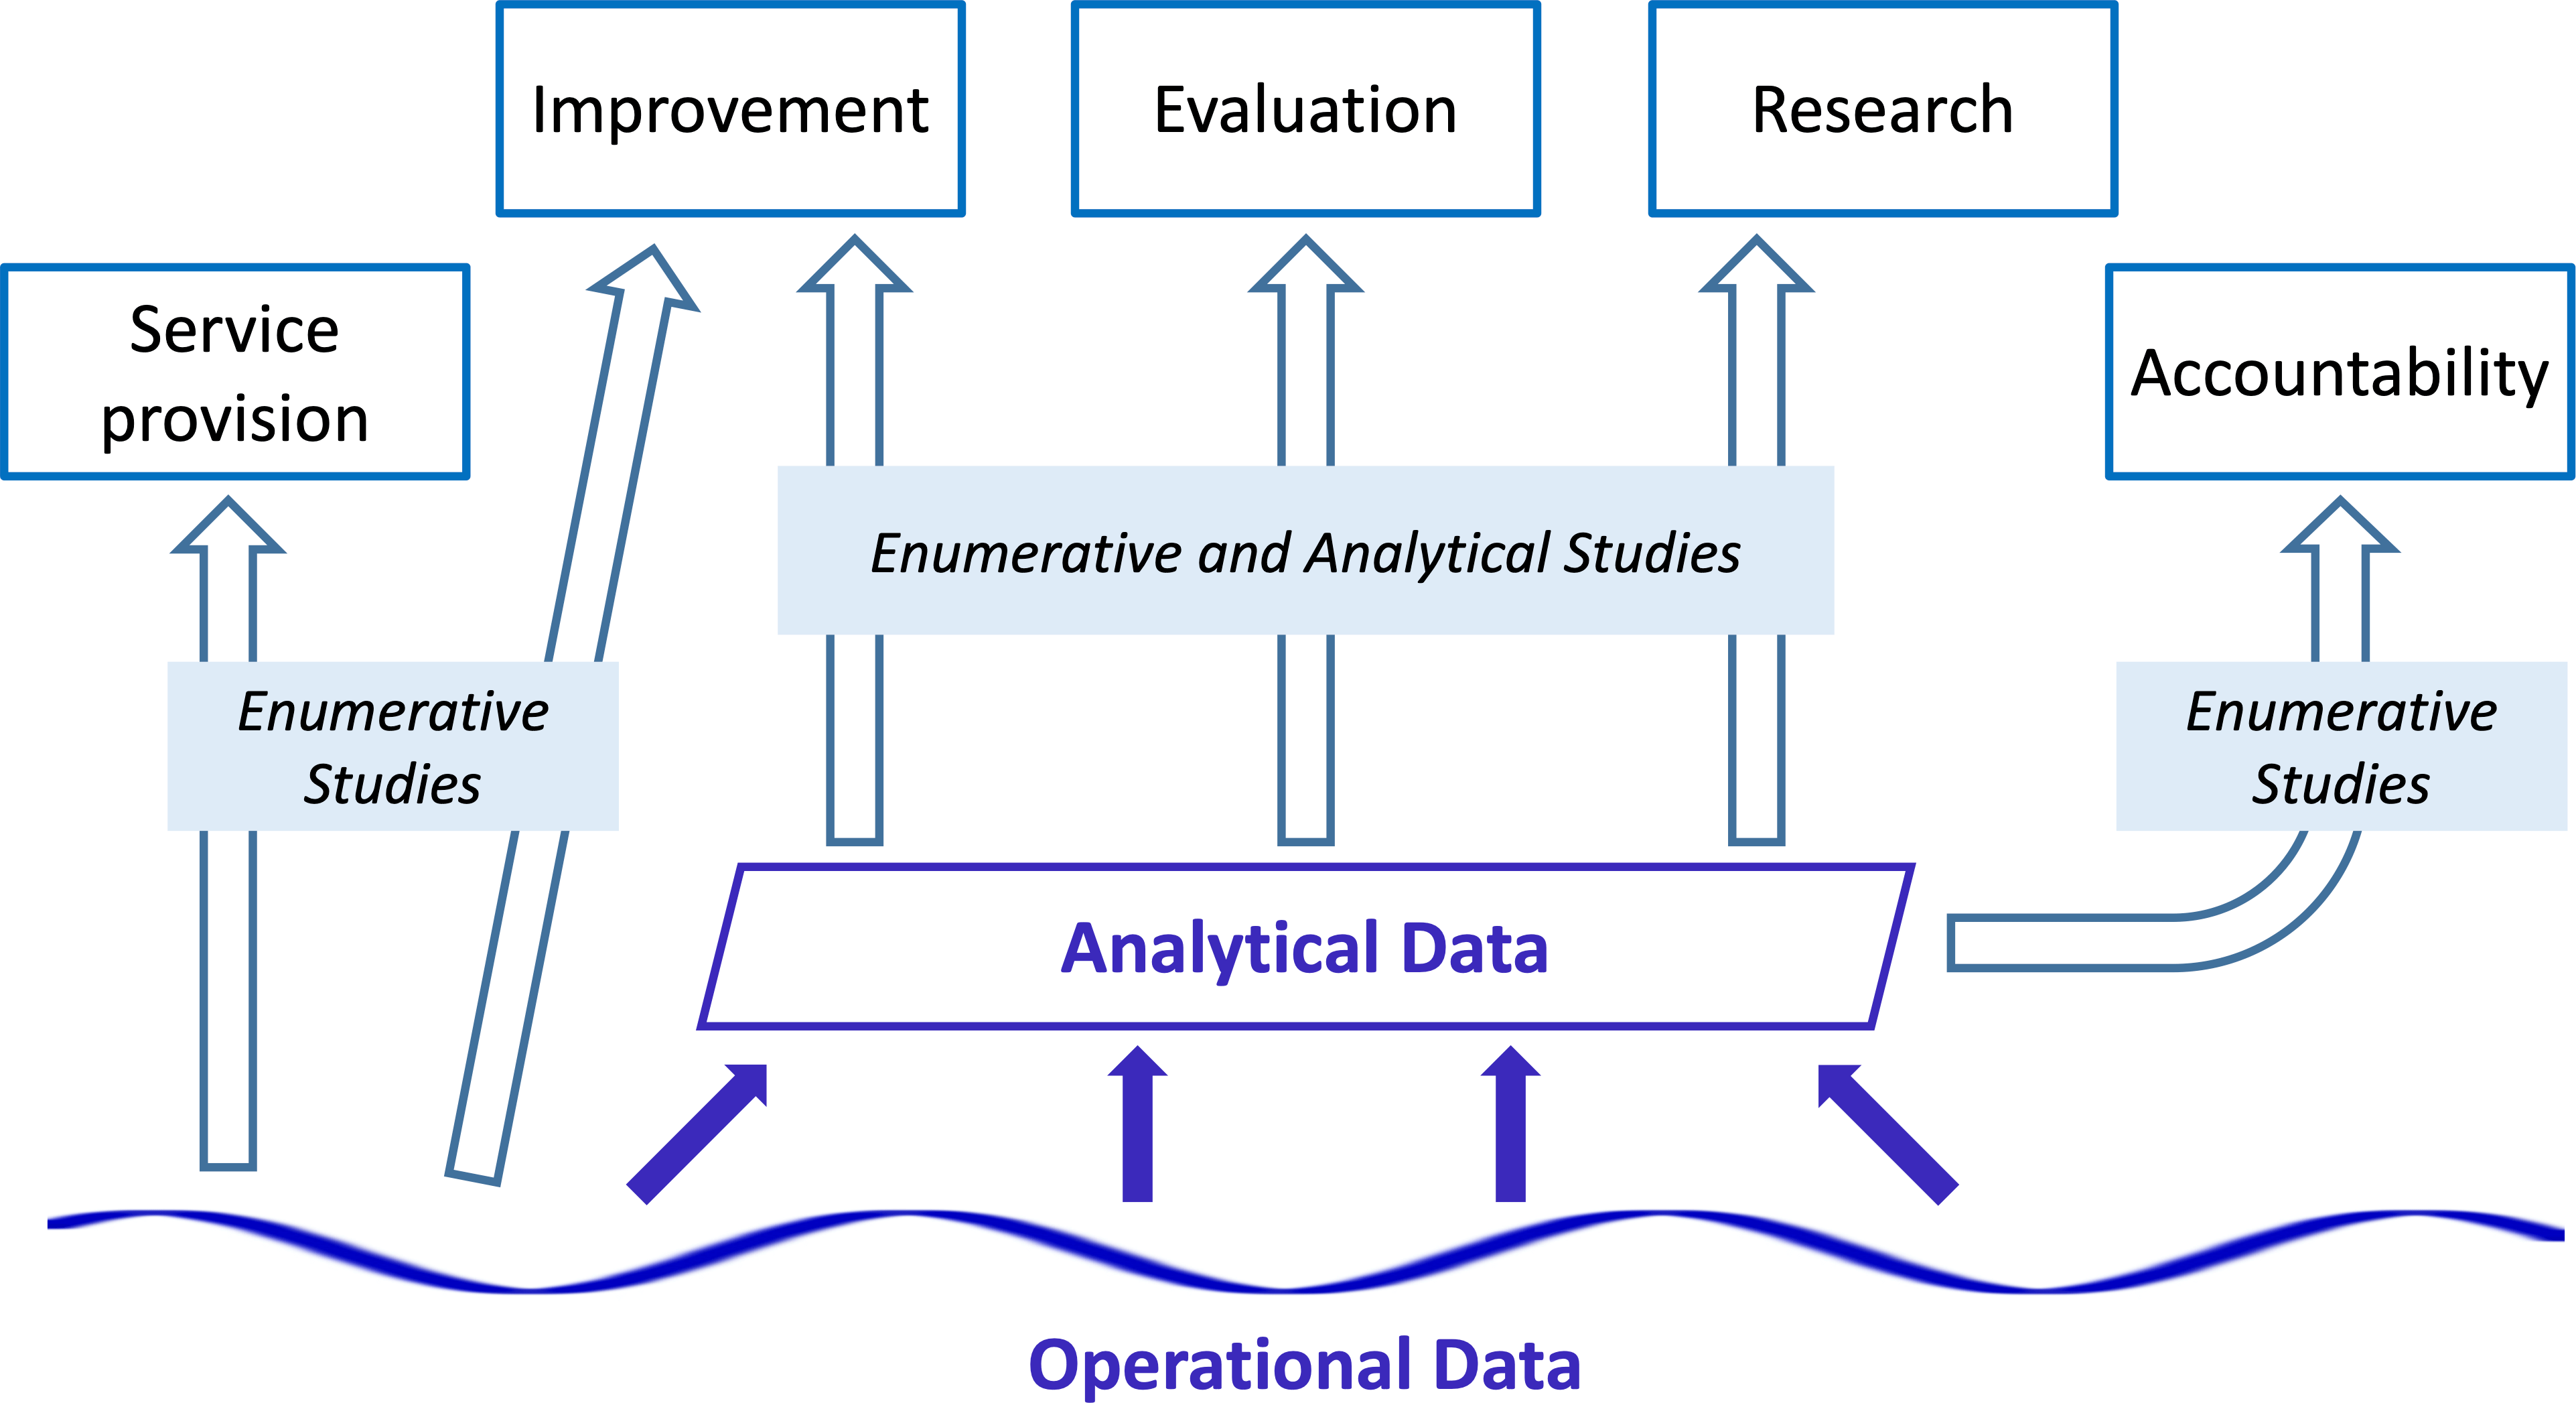
\includegraphics[width=1\linewidth]{./figures/sfusdfigure1} \caption{Relationships between purposes of data use, study types, and the data systems that support them}\label{fig:sfusdfigure1}
\end{figure}

Ultimately, the differentiation between operational data\index{Operational data} and analytical data\index{analytical data} is important for the usability of data, not only in terms of researchers accessing data but also regarding whether the data can be used to generate reliable and meaningful evidence for district decision-making.\footnote{Accountability and improvement work have largely been implemented internally within the district.} Thus, any data-sharing arrangement must closely manage the process of generating analytical data from operational data to ensure high-quality data throughout.

\hypertarget{processes-for-compiling-operational-data-and-converting-to-analytical-data}{%
\subsection{Processes for Compiling Operational Data and Converting to Analytical Data}\label{processes-for-compiling-operational-data-and-converting-to-analytical-data}}

Although SFUSD has been working toward streamlining the data systems and workflows in the district, it does not yet have a tightly integrated and coordinated system for collecting and housing analytical data. In recent years, the district has been consolidating various disparate systems and standardizing practices surrounding data. In addition to technical changes in the software, these efforts have also included refining the social infrastructure, such as establishing clear data governance and crafting shared definitions and approaches for data analysis. Given the diversity of the data systems, the data transfer arrangement from the district to the university has consisted of two tracks: one highly systematized track from the main student information system\index{student information system} (SIS) and a second, less regularized track for various data beyond those stored in the SIS, which necessitated the establishment of new routines.

The standard track has a well-established workflow for extracting from the operational data and generating analytical data files. Every fall, an analyst at SFUSD's research office pulls and processes a set of data from a Microsoft SQL database server, which contains tables extracted from the district's SIS for the previous school year. These are internally referred to as the RPA tables\index{RPA tables}, named after the district's research office. The data capture snapshots from the end of each school year. For example, the data for the 2018--2019 school year would be prepared in fall 2019. The elements include various student-level data, such as their enrollment, courses, grades, and assessment results. These data elements are documented in internal codebooks, which list the variables included in each data file, the description of the field, and their possible values. The district shares this codebook with the CEPA Data Manager and Stanford researchers. Similarly, the employee information system\index{employee information system} (EIS) database has its own set of documentation that comes from the Human Resources division.

The second track, for data outside the primary and established mode of transfers described above, has become more refined in recent years. Nevertheless, the workflows for generating analytical data for these are still less institutionalized than the main track. The current routines require the Supervisor of Analytics at SFUSD's research office, who manages the district's data sharing processes, to work with data owners around the district to obtain, process, and transfer the data. Data owners would (1) use the applicable aspects of the SIS, thereby making their data accessible to the research department, or (2) periodically transfer data to the research department. The Supervisor of Analytics documents the definition, the population, and the value descriptors in collaboration with the data owners and shares the documentation with the university.

This second track of compiling and processing data became necessary over time due to the proliferation of data systems and underutilization of SIS functionalities. This led to numerous data elements contained in the umbrella DUA being located with specific departments and staff that oversaw, inputted, or generated the data. Thus, the first step toward making data usable was to track down and obtain data elements from the appropriate owners. In 2017, when the Supervisor of Analytics took on the role of coordinating data exchanges on the district side, the investigation took a significant amount of time and effort. Examples of these investigations included compiling data from the Early Education Department\index{Early Education Department} (EED) (serving children ages 3 months through 5 years), which uses a different SIS due to distinct reporting and management needs, and the homelessness data\index{homelessness data}, which involve multiple definitions of homelessness and service providers.

The operational data collected in these manners require various processing to be converted to analytical data. Three generic types of processing are necessary for the data gathered from the district's departments: restructuring data extracted from different systems to make them congruous with the main data; compiling, comparing, and contrasting different methods and data tracking the same phenomenon; and eliminating data errors. We discuss an example for each of these here. First, EED's SIS has its own particular schema for organizing student data. In that system, the data are structured differently, with column headers and value descriptors that are distinct from the district's main SIS. For example, the sets of values capturing students' race/ethnicity differ between the systems. Second, data about homelessness demonstrate another type of gap between school operations and education research. The district maintains two sets of data for students' housing statuses. One is based on students' participation in the housing program administered by the city and the county. The other, following the state's accountability reporting requirements, is based on students' housing arrangement at home. However, research based on a student-year unit of observation requires an indicator of students' annual status, and neither data set comprehensively captures students' challenges; both can vary within a school year, and the two track different aspects of students' experiences. The district does not choose which series to use. Instead, it makes all the various metrics available to the CEPA data warehouse\index{data warehouse}. Lastly, even the official state assessment results files---such as those for the English Language Proficiency Assessments for California (ELPAC, formerly known as the California English Language Development Test)---might contain multiple records for some students that must be systematically unduplicated.

Analytical data generated through this second track are not documented in the main internal codebook associated with the RPA tables\index{RPA tables}. The district owners of each set of data provide the Supervisor of Analytics with the necessary information, who then passes it along to Stanford. Data that originate from external sources, such as the state or third-party testing services, have their own documentation prepared by the respective source. Infrequently, metadata about some variables are not yet fully documented by the time researchers request them for a project. In such cases, the project stands by while the Supervisor of Analytics works with the appropriate data owner in the district to obtain the information.

All the data throughout the district that have been obtained and processed into analytical data\index{analytical data} files through these two tracks are then transferred to the Stanford data warehouse\index{data warehouse}. Operational data\index{Operational data} used in the generation of the analytical data are not transferred to the warehouse. At the warehouse, the data undergo further structuring as described below. While the analytical data are archived at the district's research department, no process presently exists at the district to rigorously structure the archived data into a database system. This is a significant gap that should be resolved, as doing so would facilitate research and evaluation by district staff as well as other research partners beyond Stanford.

One key lesson learned comes from the variation in the Partnership's management of these processes over time. These sometimes followed a predictable schedule for data extractions and sometimes permitted ad hoc extractions for individual projects or newly-integrated data sources. These exceptions have led to complications when reconciling discrepancies in external research and internal accountability reports with partial overlap in their data source, date, or definition. The Partnership strives for greater consistency in routines for conducting, documenting, and compiling extractions from operational data to analytical data and encourage other agencies and partnerships to invest much more heavily in this area. This would ensure accuracy in the findings and promote confidence in the interpretations for action.

\hypertarget{processes-for-organizing-and-storing-analytical-data}{%
\subsection{Processes for Organizing and Storing Analytical Data}\label{processes-for-organizing-and-storing-analytical-data}}

After the operational data have been converted to analytical data, they need to be organized and stored in an accessible manner. The Stanford-SFUSD partnership established a data warehouse\index{data warehouse} at CEPA to serve this function, although the warehouse could have been set up elsewhere. The warehouse encrypts and stores the data on servers under the direct control of the Data Manager, reducing the likelihood that unauthorized users can gain electronic access to the data. While no security arrangement is foolproof, taking steps to safeguard the data is important not only because of the organization's contractual obligation to do so, but also as part of its ethical responsibility to the students and staff of SFUSD as well as to ensure that Stanford is a trustworthy research partner.

Upon being notified by SFUSD that a data transfer has taken place, the CEPA data manager\index{data manager} downloads and removes the data from the Google Suite for Education's shared drive. One of the key tasks for the Data Manager is to organize the analytical data\index{analytical data} to allow for rapid responses to researcher data requests. As of mid-2019, the warehouse uses a self-documenting folder naming system that tracks the year and month of receiving the data files and the type of data received. For example, staff data files received in April 2018 would be placed in a folder named ``201804\_Staff.'' This system is self-documenting by making it apparent which folder contains what set of raw analytical data and when the data were received. This file naming system was chosen because of the timing and frequency of the data transfers. The warehouse does not receive data sufficiently frequently where tracking the data at more than a monthly interval is necessary. The warehouse also places documentation files that accompany the raw data into the folder.

To make use of the analytical data files, the data warehouse\index{data warehouse} processes the data into master data sets as an intermediate step before providing the data to research teams. The Data Manager imports the data to Stata for cleaning and processing, with the code for the data cleaning process saved as Stata do-files (also known as syntax files). The master data files are cleaned versions of the annual analytical data that are organized into longitudinal data files and serve as the source of the data provided to researchers. This is done for the data files most commonly used by the research teams at Stanford, such as the annual student data extracts and the biannual staff data extracts. By pre-processing the analytical data from the district into the master data files, the warehouse is generally able to significantly reduce the turnaround time between receiving a data request from a research team and providing a research team with the data that they have requested. The only instance in which this does not hold true is if a research project requests data that the warehouse does not already hold and requires SFUSD to transfer the files to the warehouse specifically for that research project.

\hypertarget{legal-and-institutional-framework-4}{%
\section{Legal and Institutional Framework}\label{legal-and-institutional-framework-4}}

As alluded to above, making the school district's administrative data usable for research involves staff members in various roles, social and technical structures for collaboration, and legal arrangements to comply with systems protecting student privacy. This section first describes the current institutional set-up and some lessons emerging from its evolution, before proceeding to discuss the legal contexts and structures for sharing and using data.

\hypertarget{institutional-setup-4}{%
\subsection{Institutional Setup}\label{institutional-setup-4}}

The Stanford-SFUSD Partnership's infrastructure for sharing data involves the two partnering organizations---the school district and the university---and a facilitating third-party, non-profit organization, California Education Partners (``Ed Partners''). This section begins by describing the agency data infrastructure where the data originate; followed by the data warehouse where the data are stored; and finally, the staffing to support both infrastructures.

\hypertarget{agency-data-infrastructure}{%
\subsubsection{Agency Data Infrastructure}\label{agency-data-infrastructure}}

As described above, converting operational data into research-ready analytical data requires processing by the agency that produced the data. This motivates the need for a robust data infrastructure within the agency for organizing and maintaining the authoritative versions of the analytical data. Strengthening the upstream processes of data governance and data management within the agency would accrue benefits for all subsequent analyses, regardless of who conducts those analyses. Focusing investments downstream, in the processes of transferring data to the research partner and any corresponding cleanup of the data, would lead to other consequences. Such efforts may overlook and thus inherit the challenges that result from inconsistencies in the agency's data infrastructure. This section discusses some key issues for strengthening the upstream portion of data systems within the agency.

The first issue to consider is how much and in what way the agency might centralize the internal data systems. In school districts, including SFUSD, data systems likely proliferate and diversify over time as different departments procure tools to best meet their needs. Such proliferation poses a challenge when operational data\index{Operational data} from various sources need to be compiled and transformed into analytical data\index{analytical data}. One approach to minimizing this challenge is to consolidate and reduce the number of distinct systems. Other advantages of this may be in making the data more available for on-demand analysis and better aligned with other data systems. While this approach would be the most sustainable, it may require some investments of time and money to establish, and it may not be suitable if a select few platforms for collecting and managing data cannot meet the diverse needs of the agency. Thus, an alternate approach might be to centrally coordinate the efforts of data teams dispersed throughout the agency. This is the approach SFUSD took with some limited success. The Supervisor of Analytics collaborated with other data leaders throughout the district to develop a common culture and practices for working with data. The shared language and relationships among analysts facilitated conversations when compiling the decentralized data.

The second and related issue is to invest in data governance and data quality management within the agency. Establishing sound data governance takes time, because it requires identifying appropriate staff to own, steward, and manage the data, as well as devising processes for gathering, inputting, processing, and analyzing data. While implementing and improving data governance may be a resource-intensive investment, it ultimately offers greater flexibility and sustainability over time, as robust processes and documentation for managing data quality can help mitigate challenges arising from multiple and new data systems, as well as staff turnover.

Lastly, there are smaller investments that the agency partner can consider making beyond these two larger investments. One is to systematically create snapshots of operational data at fixed time points throughout the year. In the school context, the two main time points are the census day (the state-mandated day on which the count of students enrolled at each school site is taken) and the last day of the school year. These snapshots should be created from as many data systems as possible throughout the agency, so if a research question requiring some variables arises in the future, necessary analytical data files can be generated. The other strategy is to systematically record and document all notes about data. Such records would entail notes not only about the source, date, and definition of measures, but also any errors discovered and how they are addressed, changes in the definition or methodology, and how these impact downstream data analysis.

While these are simpler strategies that invest in the agency partner's internal data capacity rather than streamlining decentralization and improving data governance, they still require substantial investment into the hardware and software for archiving data and require appropriate staffing. A staff person would need to (1) collaborate with appropriate departments and teams to coordinate the periodic archiving of snapshot data, (2) compile and organize data on a durable server using software that can accommodate different types of data, and (3) document issues and fixes as well as the typical codebook information. In this respect, agency staffing is a critical investment for prospective partnerships to consider.

\hypertarget{data-warehouse}{%
\subsubsection{Data Warehouse}\label{data-warehouse}}

The initial choices that the Partnership made focused on addressing the demands for data from the district. Rather than investing in the upstream (the district's data infrastructure) the Partnership started by establishing a warehouse of SFUSD data which Stanford faculty could more easily access. The decision to host the warehouse at Stanford rather than at SFUSD was due to a number of factors including active faculty research projects, pre-existing infrastructure at Stanford, and an institutional commitment to creating and sustaining a long-term data warehouse\index{data warehouse} within CEPA. A number of faculty already were doing work with SFUSD and had access to large portions of the SFUSD administrative data sets. Second, CEPA had a number of data managers and analysts on staff who were previously familiar with the SFUSD data. Finally, faculty within CEPA work with several research partners and were committed to building a warehouse that would support research with multiple school districts; they were happy to include the data infrastructure for the Stanford-SFUSD Partnership as well.

While the Partnership's focus on refining the data-sharing infrastructure has contributed to its continued productivity, developing these infrastructures has been a double-edged sword. A positive aspect is that a process is now well established for researchers and practitioners to create projects collaboratively so that a list of appropriate data elements can be identified and arranged. A less favorable development has been how the initial choice about the infrastructure constrained potential choices about it down the road. Whereas the infrastructure was developed as part of Stanford's interests in conducting research at SFUSD and other agencies, SFUSD's needs for data sharing with other institutions have likewise grown. One specific challenge emerged in the context of anonymizing student identities. From the onset, the last part of data processing and algorithmic replacement of the student ID numbers took place at the CEPA data warehouse. Over time, this has complicated data-sharing agreements, as some of Stanford's researchers have relocated to other institutions while continuing their projects with SFUSD data and SFUSD's partnerships with researchers at other institutions have expanded. New and young partnerships should consider how the research and partnership needs of the agencies may evolve in the future when building their data infrastructures, as initial investments will limit future choices.

For a district with partnerships across multiple institutions, hosting the data warehouse\index{data warehouse} at the district would bring additional benefits to data quality and management. One reason is that it would ensure maintaining all the master research data files at the district without subsequent processing occurring elsewhere. In such an arrangement, the district---the data-producing agency---would continue to own the authoritative analytical data files, managing any necessary corrections as well as any procedures for converting operational data into analytical data. Increasing the efficiency of data management can then improve data accuracy by removing the need to review and update multiple versions of the same data (i.e., at the district and then at the warehouse). Maintaining a single analytical database for all external research and evaluation would improve consistency across multiple partners whose analyses may draw upon overlapping sets of data. It could also streamline communication upon creating standard metadata documentation that could be easily shared across multiple partners. In addition, having such research-ready data housed internally would facilitate more rapid internal analysis by district staff in conjunction with the analysis done by external researchers. With improved consistency of data between research and accountability reporting, this increases transparency and trust of the research. Such internal analyses could further strengthen district leaders' and practitioners' understanding of the data, as well as the district's ability to use the resulting research.

One new challenge that would emerge from hosting the research data files at the data-owning agency would be how to manage the workload of data requests and transfers. When the volume of requests from a research institution becomes sufficiently high, it may become worthwhile to mirror the entirety of data files at the requesting institution, and dedicate a data manager at that institution to fulfill data requests originating from there. While the infrastructure for exchanging data would look very much like the existing arrangement between SFUSD and Stanford, the final data processing would be completed at the district, so that the district owns the official data and the external warehouse would only serve as a mirror.

More generally, new and prospective partnerships should consider the following questions when deciding how to establish their data infrastructures:

\begin{itemize}
\tightlist
\item
  What is the expected longevity of the partnership?
\item
  How likely are the researchers at the research organization to move to different institutions?
\item
  What is the agency's anticipated number of other external research partners?
\item
  What are the costs of establishing and maintaining multiple warehouses or mirror sites?
\item
  What might be the time costs of managing multiple, disparate procedures for de-identifying/scrambling data?
\item
  How might the agency's needs for research change over time to include greater diversity in methodological and content expertise, potentially at different institutions?
\item
  What might be the necessary investment in building agency capacity for maintaining data infrastructure and managing data transfers?
\end{itemize}

A small agency that plans to have the bulk of its analysis conducted by a single external partner may find it more efficient to invest in the downstream processes of data transfer and cleanup. In contrast, an agency that anticipates developing long-term partnerships with researchers across multiple agencies or that conducts its own analyses in-house may reap greater benefits from investing in upstream data management and governance within the agency.

\hypertarget{staffing}{%
\subsubsection{Staffing}\label{staffing}}

Staffing the data-sharing infrastructure appropriately is critical to the fluid functioning of the arrangement, along with having clear processes and workflows. At SFUSD, the supervisor of research and evaluation\index{supervisor of research and evaluation} in RPA manages the overarching process of co-designing, vetting, and approving research projects as well as guiding researchers and practitioners to interpret and act on the findings. Since 2017, the supervisor of analytics\index{supervisor of analytics} in RPA has been the point person for managing and housing SFUSD data for research, devoting about 20 percent of the role's time to data management, including supplying data to Stanford and other research institutions. For Stanford, the data manager\index{data manager} at CEPA\index{CEPA} is the point person for managing and housing SFUSD data within the university, with about 50 percent of their allocated time focused on maintaining the data infrastructure for the Stanford-SFUSD Partnership. For Ed Partners, the Partnership director\index{Partnership director} of the Stanford-SFUSD Partnership manages day-to-day activities, ensures the agreements and operations are properly functioning to support the data exchange, and supports the Supervisor of Analytics and the Data Manager in the data compilation and exchange. The Partnership director devotes about 10 to 20 percent of the role to supporting data infrastructure.

Having a single dedicated data contact person at the district has been helpful for facilitating data exchanges. Previously, the supervisor of research and evaluation\index{supervisor of research and evaluation} and the Partnership director\index{Partnership director} managed DUAs and investigated data issues without having in-depth knowledge about effective data management practices or the district's data systems and issues. Under the new infrastructure, the supervisor of analytics\index{supervisor of analytics} at SFUSD and the data manager\index{data manager} at Stanford communicate routinely and manage inquiries at their respective institutions.

The Stanford-SFUSD Partnership experience, however, raises a potential question for the sustainability of the staffing infrastructure. In August of 2019, both the supervisor of analytics\index{supervisor of analytics} and the data manager\index{data manager} left their respective positions and institutions. Filling the vacant positions subsequently required approximately two months at SFUSD and one month at Stanford. While this turnover has provided an opportunity for the Partnership to review and improve the robustness of its data management processes, it does pose a strain on both institutional partners and on research projects. In addition, because of the gaps in continuity, such churn also requires training new staff to learn highly contextualized knowledge at their respective institutions.

This raises three important questions for prospective partnerships to consider for staffing the data exchange work stream. First, how many staff members will be involved and with which institution will they be affiliated? The Partnership has designated staff members at both institutions to support the data transfer, each responsible for communicating with stakeholders at their respective institutions. For partnerships with multiple data managers, how might the roles and responsibilities be distributed efficiently across institutions? Similarly, for government agencies and research organizations with multiple partners, how might they allocate staff and responsibilities across their multiple partnerships? What are the implications of these circumstances for the number of data managers hired, and whether they reside at the agency or the research organization? How much data sharing would have to happen to justify the cost of hiring a data manager at each institution? The considerations behind the choice of the location of staff would echo those about the location of the CEPA data warehouse (discussed \protect\hyperlink{data-warehouse}{above}).

Second, how might the staff members obtain the knowledge and skills necessary to facilitate smooth data sharing? These responsibilities demand a blend of technical skills, interpersonal skills, and contextual knowledge---a combination which requires considerable training and experience. The relevant technical expertise includes not just skills with data management, but also understanding of social science research methods. Interpersonal skills encompass the ability to communicate clearly and efficiently with practitioners and researchers about issues related to how the data were collected and how they will be used for the research. Moreover, data managers benefit from being deeply embedded in their respective contexts to be acculturated and understand the structures and norms guiding how their organizations function.

Third, how should partnerships recruit, train, and retain staff members with the necessary background to minimize turnover and repeated training? How should they manage through staff transitions? What alternate arrangements might they consider for distributing responsibilities across roles to maximize the value from these specialized skill sets and interests? These are critical considerations for partnerships, both because personnel constitute significant ongoing costs and because they influence the social infrastructure and relational dynamics.

\hypertarget{legal-context-for-data-use-4}{%
\subsection{Legal Context for Data Use}\label{legal-context-for-data-use-4}}

In addition to the umbrella warehousing agreement between Stanford University GSE, CEPA, and SFUSD, the partners also created a project-level DUA template\index{DUA template}, which Stanford researchers could easily fill out when submitting data requests to SFUSD. With this DUA template, the Stanford and SFUSD legal teams would not need to review every project DUA, as the template maintained consistent legal language agreed upon by both Stanford and SFUSD legal counsel. Both the umbrella agreement and DUA template are reviewed and edited every three years.

The elements included in the original umbrella agreement, which warehoused the SFUSD data at Stanford, were compiled according to the data needed for existing research projects between Stanford researchers and SFUSD administrators. Based on the original negotiated projects, these data included student and staff identifiers that are anonymized and scrambled for each project, K--12 student data, early education data, staff data (teachers and principals), and other types of student and school level data allowable by the Family Educational Rights and Privacy Act\index{Family Educational Rights and Privacy Act} (FERPA). Currently, the umbrella agreement does not include survey data, which are instead maintained by researchers for their individual projects. One variable that is commonly included in other districts' DUAs for research, but which SFUSD does not share with any researchers, is the indicator of whether a student is eligible to participate in the free and reduced-price meal program. SFUSD does not share these data for research since California state regulations limit the use of these data solely to administer the program.

To keep the umbrella agreement updated, the Stanford research department, the Partnership director\index{Partnership director}, the SFUSD supervisor of analytics\index{supervisor of analytics}, and the Stanford and SFUSD legal departments needed to amend the agreement when Stanford research projects required additional elements. (See Appendix A for an example of the language in the Stanford-SFUSD Partnership's most recent agreements between Stanford and SFUSD.) From 2011 to 2014, the umbrella agreement was amended three times; from 2014 to 2017, it was amended once. (See Appendix B for an example of one of the amendment templates.) Similarly, project DUAs often needed to be amended to add new data elements or to extend the time frame of the research. Sometimes researchers forgot to request a variable of interest, while other times projects expanded in scope and required additional data elements not previously requested or not previously collected by the district. Therefore, SFUSD's research department and both institutions' legal teams developed an amendment template that project leaders could fill out and sign.

The benefits of the CEPA data warehouse and streamlining of agreement formation and access are threefold. First, it simplifies and standardizes research support operations for SFUSD, as they can supply data to their Stanford research partners a handful of times a year, rather than providing data for one project at a time. Second, for Stanford, this reduces the amount of time Stanford researchers wait for data extracts and provides a data manager on campus whom researchers can ask questions to help clarify their understanding of the data. Third, for SFUSD as well as the broader public and research community, increasing the efficiency of conducting this research allows more time to focus on strengthening the quality and usefulness of the research produced, to better improve district decision-making, and inform the field of education.

\hypertarget{legal-framework-for-granting-data-access-4}{%
\subsection{Legal Framework for Granting Data Access}\label{legal-framework-for-granting-data-access-4}}

To access this data infrastructure as a researcher operationalizing a project (like the ones described above), there is a set of agreements related to the data access, exchange, and use for the Stanford-SFUSD Partnership. Guiding the overall governance of the Stanford-SFUSD Partnership is what is called a handshake agreement, or a non-binding written document, which outlines the goals, activities, and commitment of resources by all the key leaders guiding the partnership: the SFUSD superintendent; SFUSD deputy superintendent; the SFUSD chief of Research, Planning, and Assessment; the Stanford GSE dean; and the leaders at California Education Partners. While this is not a legal document, it guides the governance, structures, and resources committed to the Partnership.

The three legal agreements used to guide the partnership are a data warehousing agreement between SFUSD and Stanford, referred to as the umbrella agreement above; research approval processes conducted by Stanford University's Institutional Review Board\index{Institutional review board} (IRB) and SFUSD's research department; and a project-level DUA. First, the leaders at Stanford GSE (in this case the dean), at Stanford CEPA, and at SFUSD's research department negotiate the data warehousing umbrella agreement as described above.

Second, Stanford and SFUSD both have their own review processes for research involving human subjects (see the sections \protect\hyperlink{safe-projects-7}{Safe Projects} and \protect\hyperlink{safe-people-7}{Safe People} for more detail). Stanford researchers must fill out extensive paperwork to file for IRB with Stanford; in addition, SFUSD requires all researchers to submit a separate application for district review. Over time, SFUSD has streamlined their research application and developed a more consistent review process.

Third, there is a project-based DUA template with fixed legal language, which is reviewed and approved by the Stanford and SFUSD legal counsel. This template is used to develop project-level agreements for Stanford faculty to access SFUSD data through the CEPA data warehouse. For approved projects that will use administrative data, researchers must also complete a DUA specifying the data elements and years of data they will be permitted to access. The duration of these DUAs varies by project, and researchers can amend or renew those DUAs as needed through another template with pre-approved legal language. There are strict provisions for Stanford to abide by, including SFUSD asking Stanford to destroy the data at the end of a study.

\hypertarget{barriers-and-challenges-encountered}{%
\subsubsection{Barriers and Challenges Encountered}\label{barriers-and-challenges-encountered}}

While the procedures discussed thus far generally work well, one continued challenge involves deviations from the standard process. At times, projects have bypassed or sought to bypass the official data transfer procedures. Various Stanford researchers communicate directly with SFUSD departments to address questions about the data. Prior to establishing the DUAs and strict procedures for data exchange, some departments sent data directly to the researchers at Stanford, not realizing the need to go through the district's research office and the CEPA data warehouse. When this happened, the data were frequently transferred through unsecured means, such as district staff e-mailing unencrypted/unscrambled data spreadsheets to researchers.

While this was easy and efficient for the individual departments and researchers, it sidestepped the data safeguards built into the RPP\index{RPP} and the CEPA data warehouse workflow. As noted, data were not properly encrypted or transferred in a manner to properly protect the personal information of the people represented in the data. Further, such transfers also made it difficult for the CEPA data warehouse to support the researchers in the future if and when they approached the warehouse for (1) subsequent longitudinal data to join to their original data or (2) any issues about the data quality or definitions. This also complicated efforts to maintain consistent analytical data, as extractions occurred at irregular points in time and were not documented routinely.

Although such deviations have been rare, the demand for them typically has arisen out of two sources: urgency or lack of awareness on the part of practitioners or researchers. The most prevalent has been lack of awareness of the standards for data exchange among individual departments and researchers. For instance, researchers and district staff may not understand that all projects need centralized approval not only from Stanford's Research Compliance Office IRB\index{Institutional review board} but also from SFUSD. In other cases, SFUSD staff or Stanford researchers may seek to expedite the data transfer for reasons such as the district wanting results for time-sensitive policy decisions or Stanford researchers needing to make deadlines for publications or conference submissions. Such urgency has sometimes resulted in the data owners/researchers bypassing the established process. For either of these scenarios, the Partnership has endeavored both to halt the irregular transfers and to strengthen the knowledge and understanding among staff and researchers.

Another challenge to the established and evolving data-sharing arrangement has emerged from the success of its long-term functioning. Over time, Stanford researchers (both faculty members and graduate students) have moved to other institutions but sought to continue their research using SFUSD data. Because the data-sharing infrastructure is designed only to serve researchers working within the Stanford-SFUSD Partnership, maintaining an appropriate arrangement has been a challenge. The two stopgap remedies that the Partnership has implemented thus far are to (1) create a multi-party data-sharing agreement between SFUSD, Stanford, and the third-party academic institution or (2) require the researchers at a new institution to be sponsored by or to formally collaborate with a current Stanford faculty member. Both approaches are inelegant solutions to the need for efficient and effective data sharing. This issue is revisited/readdressed at the end of the chapter.

During the earlier years of the Partnership, each DUA was drafted, negotiated, and executed anew, as noted above. SFUSD's Legal Department then had to approve each DUA, which impeded the efficiency of the data exchange process. Eventually, the Partnership invested time into creating a DUA template with standardized language approved by the legal teams on both sides. Now, the template provides common and consistent provisions for data sharing, and the researchers need only fill in their project details and requested data elements. Furthermore, the agreements can be approved without requiring any attorneys' signatures, significantly speeding up the administrative process. Any research partnership that will work on multiple projects over time should invest in creating such a DUA template in the preliminary stages.

\hypertarget{protection-of-sensitive-and-personal-data-the-five-safes-framework-4}{%
\section{Protection of Sensitive and Personal Data: The Five Safes Framework}\label{protection-of-sensitive-and-personal-data-the-five-safes-framework-4}}

\hypertarget{safe-projects-4}{%
\subsection{Safe Projects}\label{safe-projects-4}}

In addition to requiring documentation of university IRB\index{Institutional review board} approval prior to reviewing any research projects conducted in the district, SFUSD's research department also engages additional scrutiny to ensure safe projects. As mandated by FERPA\index{Family Educational Rights and Privacy Act}, SFUSD's research department requires all research requests using administrative data to establish a formal legal agreement specifying the parameters of the data sharing. These parameters are the purpose, scope, and duration of the study; the data elements needed; and the research organization that will receive and secure the data. SFUSD applies these expectations to all research studies, even when administrative data are de-identified; this is due to the potential for individual student-level data to become identifiable upon combining different student and school characteristics and due to the desire to closely monitor external data-sharing given the risks posed with sharing data.

While the function of requiring documentation of external IRB\index{Institutional review board} exemption or approval is to ensure adherence to ethical standards for all research, whether federally funded or not, the purpose of SFUSD's internal review before approving research applications is to evaluate the compatibility with district priorities. Projects must demonstrate their benefit to the district and justify their need for district administrative data. The expectations SFUSD applies are summarized as the alignment, benefits, and costs (ABCs) of the proposed research. First, the research must be closely aligned with the district's strategic plan and learning agenda. Second, the project must be likely to yield benefits to policy or practice, meaning that key district decision-makers must be prepared to use the research results to yield a positive impact on relevant stakeholders with the benefits being sustainable. Third, conducting the research must incur minimal costs, in terms of time, resources, and burden to people. Costs may include the efforts needed to obtain informed consent prior to collecting primary data or releasing personally identifiable secondary data, the time required to collect and process the data, or ethical considerations regarding who bears the burden as the subject of the research.

SFUSD evaluates these dimensions by surveying the relevant district leaders most closely connected to the topic of the study who would sponsor the research, along with having its research department staff review the proposal to determine whether the design is likely to provide valid and useful findings on a timeline that can help inform the desired practical decisions. This internal review also includes a close inspection of the data elements requested in order to confirm their availability and their necessity to answer the research questions of interest. Thus, SFUSD maintains a higher bar for research approval than required by federal code.

Prior to submitting applications, researchers are instructed to consult the district website for information on its long-term vision and current strategic plan. In some cases, researchers may have the opportunity to engage directly with district staff during the development of a potential research project, whether initiated by the district in seeking research on a particular question or initiated by a researcher pitching a specific idea. Thanks to additional funding for the research-practice partnership, Stanford researchers have greater access to such guidance through the Partnership director as well as an annual grant mechanism to incentivize Stanford-SFUSD research. One challenge is that this creates inequities between research organizations. SFUSD's research department is working to correct this through stronger institution-wide messaging both within and beyond the district about research interests and opportunities, circulating requests for proposals, formalizing more of its relationships with other partners, and establishing standard processes to use across partnerships for developing research ideas.

SFUSD's research department is also continuing to strengthen its practice of assessing the cost-benefit tradeoffs of research projects. While many projects can be executed with minimal efforts using the existing archive of administrative data, other projects accrue significant costs in primary data collection, linking primary data with secondary administrative data, or processing and manipulation of administrative data. In such cases, the potential benefit of the research may be offset by the costliness involved in obtaining or providing the data. SFUSD's research department has been exploring methods for quantifying these costs more systematically, as well as guiding district sponsors to consider the opportunity costs of engaging in research projects prior to committing their support. As described further under the section Metrics for Measuring Success, the Partnership is simultaneously seeking to improve the measurement of benefits. With the field of scientific research developing better metrics of success for research impact and RPP\index{RPP} effectiveness, the Partnership anticipates piloting and adopting some of these measures, along with other methods for assessing the use of research evidence. Within SFUSD, the Partnership is working to capture more consistent documentation of how research and data are used to inform practice in order to motivate greater selectivity and efficiency in efforts, including opportunities to better support the progress of active projects. The Partnership hopes to further systematize the analysis of such costs and benefits during the project development phase.

\hypertarget{safe-people-4}{%
\subsection{Safe People}\label{safe-people-4}}

Stanford University researchers who wish to utilize SFUSD administrative data for their prospective projects must fulfill several requirements prior to obtaining approval from SFUSD and receiving their data. The first requirement for researchers is to complete Stanford's human subjects training. In the event non-Stanford researchers are included on a project, they can complete their own institution's human subjects training, contingent upon the approval of the Stanford IRB\index{Institutional review board}. Stanford participates in the Collaborative Institutional Training Initiative (CITI) Program, which offers a certification course in human subjects research to familiarize all non-medical principal investigators and research staff about the Common Rule and IRB requirements. Researchers must complete the course prior to being added to an IRB protocol at Stanford, which SFUSD requires for approving a project proposal and DUA. All members of a project must be listed in the IRB protocol.

Separate from the general Stanford IRB\index{Institutional review board} requirement, Stanford researchers who receive data from the data warehouse must sign an internal access agreement that outlines their responsibilities and acknowledges that they may be held personally liable for any financial costs incurred due to a data breach for which they are responsible. The Data Manager tracks these internal access agreements and ensures that each member of the research team has completed their access agreement before transferring the data to the researchers. Once the data have been transferred to the researchers, it is the responsibility of the principal investigator to maintain data security and safety and ensure that their research staff are in compliance with the conditions set in the access agreement. As these conditions also reflect requirements set forward by Stanford University's IT security requirements, compliance tracking is left to Stanford GSE's IT staff as part of their routine auditing. To increase the transparency of all who might access and work with the shared data, starting in late 2019, the principal investigators are required to list the names of all staff anticipated to work with the data in appendices to the project-level research application and DUA.

In 2019, with an increasing number of alumni students and faculty with ongoing research projects utilizing SFUSD data, Stanford GSE and SFUSD leaders initiated a refinement of the process to more closely monitor non-Stanford researchers continuing their projects. Stanford and SFUSD developed a third-party agreement that alumni and Stanford collaborators could sign if they continued to work on projects with SFUSD. These alumni and collaborators would still need to maintain a Stanford sponsor and Stanford IRB to access the data for their projects. The template for these third-party agreements is included in Appendix A.

\hypertarget{safe-settings-4}{%
\subsection{Safe Settings}\label{safe-settings-4}}

The Partnership has three separate settings to consider for security: data at rest\index{data at rest}, data in use\index{data in use}, and data in transit\index{data in transit}. The storage of the data at the CEPA data warehouse\index{data warehouse} and the storage of the researcher-accessible data pertain to data at rest and data in use. The mechanism for transferring data between SFUSD, the CEPA data warehouse, and the researcher pertains to data in transit.

The warehouse stores the data received from SFUSD on an encrypted desktop computer with two hard drives configured in a mirrored array, to limit the possibility of data loss in the event of a hard drive failure. An additional backup of the data is kept on an encrypted external storage drive that is kept in a locked cabinet; the backup is scheduled for each time the warehouse receives data from the district. Keeping the data files off of servers that are outside the direct control of the Data Manager reduces the likelihood that unauthorized users can gain electronic access to the data. Encrypting all of the computers and drives where the data are stored reduces the possibility that an adversary can access the data even if they gain direct physical access to the computer. Both the original analytical data and the prepared master data are stored locally on the encrypted warehouse computer and backup drive. However, the syntax files used to prepare the master data are backed up onto Stanford servers, as the syntax files themselves do not contain any sensitive information.

On the researcher side, the standard DUA template used by each research project specifies the appropriate storage mechanisms for handling the data. Separately from the DUA requirements, Stanford IT also maintains a \href{https://uit.stanford.edu/guide/riskclassifications}{data risk-classification system} for all data stored on university systems with corresponding access and storage requirements for each type of data. SFUSD data are classified as high-risk data due to the legal requirements for protecting the data and the requirement to report any breaches to SFUSD, which is a government actor. In practice, the dual requirements from the DUA and Stanford risk-classification means that researchers must store the data on Stanford servers or specific cloud services approved by Stanford University IT. Access to the storage location is provisioned by the Stanford GSE IT department via Stanford single-sign-on user accounts. Stanford-based researchers have accounts as a matter of course, while guest accounts can be provided in the event that non-Stanford-based researchers are collaborating on a Stanford-based project. The data should only be accessed from computers that utilize Stanford BigFix (a centralized operating system patch management service) and whole-disk encryption. Neither Stanford nor SFUSD place any restrictions on the location from where researchers can access the data, the software researchers use, or analysis methods.

Transferring data from SFUSD to the CEPA data warehouse\index{data warehouse} and from the CEPA data warehouse to researchers utilizes the same service. The CEPA data warehouse maintains Stanford-provisioned Google shared drives, which are made available by an institutional contract between Google and Stanford University and approved by Stanford University's IT department for handling high-risk data; access is granted to the appropriate directories for SFUSD staff and Stanford researchers. One shared drive is used to transfer the complete analytical data from SFUSD to the CEPA data warehouse and to transfer researcher-generated files back to SFUSD as requested. Only SFUSD staff (including the Supervisor of Analytics, and any additional staff as requested by SFUSD) and the Data Manager have access to this shared drive. Each research project has its own separate shared drive for data transfers to and from the CEPA data warehouse; access is provisioned to research staff included on the project DUA.

Between 2014 and 2019, the CEPA data warehouse\index{data warehouse} used a secure file transfer protocol\index{secure file transfer protocol} (SFTP) server to handle data transfers. The switch to Google shared drive was prompted by a Stanford GSE IT department security analysis of its existing infrastructure alongside the planned shutdown of the SFTP server. The server was maintained by Stanford GSE IT staff, while the Data Manager had administrative privileges to manage user access. The organization of the server was identical to the current arrangement. Prior to 2014, data files were transferred physically from San Francisco to Stanford on CD-ROMs. Taking advantage of existing and well-established technologies has helped make data sharing in the Partnership much more efficient and secure than before.

One future goal of the SFUSD-Stanford partnership may be to decentralize the fulfillment of data requests such that researchers can generate custom datafiles on demand through an automatic interface. Such web applications already exist for national education data systems, such as the National Center for Education Statistics (NCES). The challenge would be in implementing a similar system for data at smaller scales, such as at the level of school districts. Coordinating on a standardized data schema---such as the Ed-Fi\index{Ed-Fi} standard in education, which provides rules for how data in education are to be formatted and exchanged between data systems---may provide the foundation for a scalable self-service data request solution in the future.

\hypertarget{safe-data-4}{%
\subsection{Safe Data}\label{safe-data-4}}

The primary concern over sensitivity of student data is embodied in FERPA\index{Family Educational Rights and Privacy Act}. The law places the authority to grant third parties access to students' educational records and data to students' guardians, which constrains the district's ability to share student-level data to highly circumscribed and exceptional scenarios. In each stage of sharing the data, from SFUSD to the CEPA data warehouse\index{data warehouse} and from the CEPA data warehouse to the researcher, the data are restricted according to the relevant DUA.

The data transferred from the district to the CEPA data warehouse includes the full set of data that may be required for SFUSD-approved research projects as defined in the CEPA data warehouse umbrella DUA. The data transferred to the CEPA data warehouse includes student names, district ID numbers, and other identifying information to facilitate the matching of data between different data sources and on behalf of research projects that collect primary data (e.g., survey responses). To enable its role as a data access provider on behalf of the district, the CEPA data warehouse DUA includes a provision that allows it to store data not explicitly listed in its own DUA if SFUSD has approved a research project to receive those data.

After SFUSD approves a research team's DUA, the data manager\index{data manager} provides the appropriate sample of data as outlined in the DUA. The research team's DUA restricts the number of years of data and variables out of each data file that they are allowed to receive for each project. For data that exist in the master data files, this is as simple as extracting the appropriate subset of data as defined in the DUA. For data that are not already in the master data or not held at the CEPA data warehouse, which are typically data rarely used by researchers, the Data Manager additionally cleans the data before initiating transfer, ensuring that only the approved subset is provided to the research team. While Stanford researchers can renew and extend their DUA if the project needs to continue past its initial agreement, they must destroy the data upon final expiration of the DUA.

Data files provided to researchers utilize district-defined student identification numbers scrambled using an algorithm developed at Stanford. Such a scheme for maintaining a consistent unique identifier for students is critical for researchers to join data from multiple sources and to carry out longitudinal studies in which cohorts of students are analyzed over time. Sometimes, for research findings to guide instruction or operations, calculated measures or analyzed results at the student level must be returned to the district. In such cases, researchers provide the data manager\index{data manager} a data file with scrambled IDs. The Data Manager \emph{unscrambles} the identifiers to restore district ID numbers before transferring the file to the district.

To comply with the law and to protect student privacy, students' and parents'/guardians' names are generally not provided to researchers. For linking data to external data, SFUSD and the CEPA data warehouse\index{data warehouse} can perform linking services on behalf of researchers. This is typically done by having the researcher provide the CEPA data warehouse with the identifying information on individuals in the data to be linked and having the data manager\index{data manager} or the supervisor of analytics\index{supervisor of analytics} perform the linkage. In rare cases, with explicit approval in the DUA, research teams may receive data such as names or official ID numbers that would enable researchers to individually identify students. Such exceptions are made only for the purposes of linking primary data to administrative data and only when all other strategies for linking the data anonymously have been exhausted. Moreover, the district requires that researchers delete the primary keys once the data files are joined.

\hypertarget{safe-outputs-4}{%
\subsection{Safe Outputs}\label{safe-outputs-4}}

District practice is to review all research products prior to submission for public dissemination. Before publishing study designs, data, or findings in open research registries, researchers must submit any data, source code, or manuscripts for SFUSD to review to verify that they have fully anonymized SFUSD data. Although analytic results are typically aggregated and reported at a level higher than individual students, these must still be reviewed to preserve anonymity. In some cases, interactions between these dimensions may yield small cell sizes or additional information is presented in the report that risks indirectly identifying individuals. Given that FERPA\index{Family Educational Rights and Privacy Act}'s standards for ``personally identifiable information'' are based on whether ``a reasonable person in the school community'' could identify the student, having district staff review the manuscript can offer this perspective to safeguard the privacy of individuals involved in the research. If projects need to provide student-level results and calculations to improve instruction or intervention, such results are shared only with district staff through the secure transfer channels rather than being publicly released.

Beyond protecting privacy, a second reason for this review is to ensure accurate accounting of the district context and practices that may be relevant in explaining the results, similar to member-checking in qualitative research. This reflects the Partnership's emphasis on the value of co-production at multiple stages throughout the research process, including presentations and publications. The Partnership's experience is that asking the administrators and practitioners most familiar with the project to review the manuscript elicits additional information that may only have been incompletely captured previously. While this is an informal expectation rather than a legal requirement, the district makes this request of its research partners as a good-faith commitment to mutual respect and partnership. It has also been found that this supports greater dissemination and use of the research, as district leaders develop a deeper understanding and appreciation of the research through increased communication about it.

A third reason for this review is to determine whether it is appropriate to identify the district in the publication. This step is important for the district to manage consistency of messaging across its many initiatives and interests, which may be competing for attention, so that communication is aligned with strategic priorities. The DUA template includes this language: ``Research Organization agrees that SFUSD shall not be named or otherwise identified in the study, unless written permission to do so is granted by SFUSD for a specific project only.''

A fourth reason for review is to check for consistency between the research results and analyses conducted either internally for evaluation or accountability or by other research teams. While the Partnership does not yet have a formal process for verifying the validity of the analyses in all research products, some ad hoc review mechanisms have emerged. However, not all publication submissions always undergo this review, possibly due to the tight timelines for submission or lack of awareness. The Partnership is working toward increasing awareness of this expectation for review prior to publication, which can strengthen not just the validity and privacy protections for the reports, but also the timeliness and breadth of awareness of the research findings. More recently, the Partnership has also begun encouraging research teams to more systematically share findings with other university colleagues and research groups as a form of informal review of the analyses. While some researchers already have internal peer review processes in their own labs and centers, this has varied across projects. Engaging all projects in such a review process is especially important for results that do not undergo publication and therefore academic peer review, as the district values the reassurance of rigor in any findings that it may use to inform decision-making.

For all of these reasons, as well as to promote greater use of the research, the Partnership encourages, but does not require, co-authorship with the district sponsors most involved in the research. The Partnership would like to improve the consistency and robustness of the processes for ensuring not just safe outputs, but useful outputs that are carefully vetted and well understood by both the research team and the practitioner partners. For the sake of validity and value, the first audience for all research products should be the members of the partnership most invested in the work with the external audience being secondary. Ideally, feedback from the peer review process should then inform subsequent conversations with the practitioner partners, so that they have the opportunity to learn from relevant interests and concerns expressed by others in the field about the research and its implications.

\hypertarget{data-life-cycle-and-replicability-3}{%
\section{Data Life Cycle and Replicability}\label{data-life-cycle-and-replicability-3}}

\hypertarget{preservation-and-reproducibility-of-researcher-accessible-files-3}{%
\subsection{Preservation and Reproducibility of Researcher-Accessible Files}\label{preservation-and-reproducibility-of-researcher-accessible-files-3}}

The data generation and cleaning process produces a set of master data sets that are cleaned versions of the yearly raw analytical data organized into longitudinal data files. The warehouse maintains all of the analytical data received from SFUSD indefinitely with the only exception being specific data files that the district requests to be deleted after transfer to researchers. The CEPA data warehouse\index{data warehouse} also maintains all of the scripts used to generate any researcher-accessible files and the version of the files last transferred to the researchers. This allows for rapid updates of the files as well as reproducing the latest version of the files transferred to the researchers on demand. In practice, this is of negligible concern regarding the master data since updates to those files are usually for additions to the longitudinal data rather than for corrections to historical data. Researchers are responsible for maintaining the data files that they receive.

\hypertarget{preservation-and-reproducibility-of-researcher-generated-files-2}{%
\subsection{Preservation and Reproducibility of Researcher-Generated Files}\label{preservation-and-reproducibility-of-researcher-generated-files-2}}

The CEPA data warehouse\index{data warehouse} itself is not responsible for maintaining researcher-generated files, as the warehouse does not have routine access to those data. Researchers are not allowed to share these data with outsiders without the permission of SFUSD. Research team agreements require that they delete their data at the termination of a research project. Historically, enforcement tends to fall on routine audits of user accounts by IT staff, although the Partnership is establishing more regular processes for following up with researchers after projects are completed to request documentation of data destruction.

\hypertarget{sustainability-and-continued-success-4}{%
\section{Sustainability and Continued Success}\label{sustainability-and-continued-success-4}}

The social and technical infrastructure for sharing data within the Stanford-SFUSD Partnership is an important piece facilitating the RPP. However, that infrastructure is embedded in a broader context that contributes to the sustainability and the continued success of the Partnership. Through outreach, researchers at Stanford and practitioners at SFUSD regularly interact with one another, strengthening relationships for collaboration. The steady funding of the key staff positions by Stanford GSE has also helped to maintain continuity. Lastly, the Partnership has continuously monitored the progress of research production and use, which is the ultimate goal of the data sharing arrangement between the institutions. These three elements are discussed in turn.

\hypertarget{outreach-3}{%
\subsection{Outreach}\label{outreach-3}}

Stanford GSE faculty and researchers learn about the Stanford-SFUSD Partnership's research priorities and SFUSD data available for that research through a number of channels. First and foremost, they learn from the Partnership director\index{Partnership director} who on-boards new faculty and hosts the Stanford-SFUSD Partnership Annual Meeting, which all faculty are invited to attend, where research produced by the Partnership is showcased. At this meeting, both the Stanford GSE dean and the SFUSD superintendent speak about how the Partnership supports their vision for their respective institutions. The Partnership director also presents information about the research conducted in the Partnership to Stanford GSE students on an annual basis. Faculty and students also can meet with the Partnership director to discuss the data in the CEPA data warehouse\index{data warehouse}, as the Partnership director has an office at Stanford GSE and is on campus one to two days a week. Second, Stanford faculty and researchers learn about SFUSD data through the CEPA data manager. SFUSD leaders and the Partnership director often send faculty and researchers to talk to the CEPA Data Manager if they have questions about the SFUSD data that are warehoused at CEPA. Third, Stanford GSE faculty and researchers also hear about the data from their peers in presentations about the SFUSD research at an on-campus annual meeting showcasing the Partnership projects. Finally, in some cases, Stanford GSE faculty and researchers communicate directly with SFUSD leaders or analysts to discuss questions about the data, such as the nuances of how the data were collected or what specific values mean, particularly when the data are owned by other departments beyond RPA.

To date the Partnership has not publicized the types of data available from the district for several reasons. Of paramount importance is promoting theory-driven research rather than studies that merely mine data for correlations. Another reason is to encourage direct communication between researchers and district leaders about the research questions and the relevant data. However, the district is now revisiting this decision in the interest of standardizing documentation and streamlining communication about the data. Continuing to maintain strict review processes can help ensure that all projects are aligned with district priorities rather than simply being an impersonal transaction of data for analysis with limited connection to practical realities or benefits.

\hypertarget{revenue-3}{%
\subsection{Revenue}\label{revenue-3}}

As mentioned above, the arrangement for data-sharing between SFUSD and Stanford University is part of a broader research-practice partnership between the district and the university. The Partnership is funded by Stanford University Graduate School of Education through private donations, and Stanford researchers are not charged a fee for their data requests. The district has occasionally charged fees for data requests for those coming from outside the Stanford-SFUSD Partnership, depending on scope and complexity. SFUSD is now implementing a more systematic and permanent fee structure for data requests from researchers outside of established partnerships with the district.

On the university side, the Stanford GSE funds roughly half of the CEPA Data Manager position as well as the hardware infrastructure necessary for the data management. On the district side, Stanford GSE funds a significant portion (about 70 percent) of the Supervisor of Analytics position. In 2018, some of the residual funds at the district were used to make significant upgrades to the hardware infrastructure at the research office for storing and archiving data.

Since 2014, Stanford GSE has made a long-term commitment to funding the Partnership through its development efforts and commits at minimum US\$500,000 a year to the Partnership for research and data infrastructure. Faculty also pursue research grants to fund research with the Partnership from private foundations and public grants offered through the US Department of Education, which also provides steady, although variable, funding for partnership research.

\hypertarget{metrics-for-measuring-success}{%
\subsection{Metrics for Measuring Success}\label{metrics-for-measuring-success}}

Together the SFUSD research department and Partnership director\index{Partnership director} monitor progress and measure success in several ways. Beyond counting access to data, the SFUSD research department and the Partnership director are most interested in the quality and impact of the research, particularly on SFUSD policy and practice. The SFUSD research department and Partnership director monitor access to ensure that the research projects are mutually beneficial to both the faculty and the district leaders involved and that the research meets a certain level of quality; the research has the potential to produce generalizable research that influences the field of education as well as producing research that informs decisions by SFUSD district leaders. While the Partnership has not yet adopted a formal measurement model, the approach is compatible and overlaps with SAGE Publication's \citeyearpar{sagepublishing2019} models of research impact and Henrick et al.'s \citeyearpar{henrick2017} framework for assessing RPP\index{RPP} effectiveness. In particular, the Partnership attends to academic and practical outcomes and shifts in understanding of research.

First, Partnership outputs are measured by examining each project's research products. External products may include peer-reviewed publications, policy briefs, conference presentations, and other reports, while internal products may include informal presentations and write-ups.

Second, the impact of the research is measured not just on the field but more immediately within SFUSD. As noted previously, the Partnership measures broader research impact by considering the type of publication as well as its audience. For impact within SFUSD, which is what the Partnership values most highly, they look for evidence of instrumental use of research through changes in policy and changes in practice (preferably at more than one school or classroom); they then note whether these led to changes in student outcomes. Following Weiss and Bucuvalas \citeyearpar{weiss1980}, the Partnership also considers conceptual use of the research by district leaders, recognizing its importance in influencing leaders' thinking as they plan future policy and practice. The SFUSD research department sends short survey questions to school and district leaders working with researchers on the projects, both when research findings are presented and when projects conclude, to assess what leaders learned and applied from the research. The survey includes questions about the anticipated sustainability and scale of the changes to begin to assess longer-term impact. Survey questions record audience attendance at research presentations and gauge knowledge of the research project, enriching measurement of the scope of research impact. The Partnership also administers its own survey to both researchers and practitioners.\footnote{See \citet{wentworth2017} for a description of the Partnership's survey development.} Notes from these discussions also inform the assessment of how district leaders and researchers are thinking about the use of the research.

Third, the capacity to engage in partnership is tracked by monitoring the number of Stanford faculty or graduate students with completed or active projects, as well as the number of SFUSD departments and leaders engaged in the Partnership. Since 2011, the quantity of research projects that access data from the warehouse at Stanford has tripled from three projects in 2011 to nine projects in 2018. Another measure of the scope of data access is the number of SFUSD departments and the number of data elements included in the umbrella DUA, which have grown over the years as research interests and projects have increased. As another process measure, SFUSD has also recently begun gathering data on time spent on extracting data and communicating about data with researchers in the interest of optimizing research impact and efficiency.

\hypertarget{concluding-remarks-1}{%
\section{Concluding Remarks}\label{concluding-remarks-1}}

Looking across the findings of this case study of the Stanford-SFUSD Partnership data infrastructure, there is a set of implications for the field and the future of the work together. Within the Stanford-SFUSD Partnership and in other partnerships pursuing a similar data infrastructure, \emph{it is important to continually improve the ways in which data are collected and archived}. For example, in SFUSD, although spreadsheet files gathered from various departments are systematically archived on an internal server, they are not processed to create robust databases. One critical step toward pursuing this improvement is to maintain a clearer separation between operational and analytical data systems. Along with better integration of the operational data systems that sit across distinct databases in the school district departments, the Partnership would also establish firmer timelines for finalizing the extracts of analytical data from these systems. Maintaining authoritative analytical data files for research at SFUSD would also significantly improve data quality, consistency in analyses, and efficiency in data management across the multiple analysts and researchers who use those data. On the Stanford side, the data manager could implement an intermediate step of data organization and storage between the raw data receipts from the district and the master data files that are used to provide data to research teams.

As discussed above, \emph{proper} \emph{staffing and clear processes and workflows for data sharing are critical.} Ensuring that the staff who support the data transfer have the necessary knowledge and skills is invaluable for smooth data sharing. These responsibilities demand a blend of technical skills, interpersonal skills, and contextual knowledge, which is a combination that requires considerable training and experience. In the Stanford-SFUSD arrangement, the district-side data manager communicates primarily with other district leaders, while the university-side data manager communicates primarily with researchers. Embedding the data managers in their respective contexts helps with acculturation and understanding the structures and norms guiding how their organizations function.

Even with all the efforts to pursue the five safes, \emph{data managers must anticipate the possibility that other personnel may deviate from the standards of the data exchange}. Researchers and practitioners may be inclined to side-step protocols because of pre-existing relationships and the desire to expedite the data exchange. To prevent or repair issues due to such deviation, the Partnership director, district research office, or other neutral brokers can help the data managers guide the personnel back on the right track. These neutral brokers can help intervene in a politically sensitive way while explaining to the research or practitioner personnel the policies guiding data exchange and the rationale for upholding them.

Beyond merely ensuring the safety and efficiency of this data infrastructure, the Partnership believes in the importance of ensuring the usefulness of engaging in such work as the top priority. Given that the Stanford-SFUSD Partnership's driving motivation is to produce generalizable research that SFUSD administrators can use to inform future action, the Partnership continues to explore how to organize the data in service of such research and consequent learning and action. In particular, a reliable data infrastructure should (1) ensure high-quality data; (2) enable efficiency in collecting, organizing, maintaining, and sharing data; and crucially, (3) facilitate using data to connect implementation to impact across multiple levels \citep{ming2019}. These features would support conducting analyses that describe, explain, and predict causal relationships between actions and outcomes. This chapter has discussed the challenges and costs associated with data-sharing in detail; it is also critical to increase the benefits that are expected to justify those costs. The authors are eager for the field to develop expectations for data standards and infrastructures that may yield more insightful research about the actions that improve outcomes.

\hypertarget{about-the-authors-6}{%
\section*{About the Authors}\label{about-the-authors-6}}
\addcontentsline{toc}{section}{About the Authors}

\href{https://ed.stanford.edu/faculty/ebetting}{Eric Bettinger} is a Professor at Stanford University Graduate School of Education, a senior fellow at the Stanford Institute for Economic Policy Research (SIEPR), and the Faculty Director of CEPA.

\href{https://gse.berkeley.edu/moonhawk-kim}{Moonhawk Kim} is the Director of Research-Practice Partnerships and Community Engagement at the Graduate School of Education, University of California Berkeley. He worked in the RPA division at SFUSD from May 2016 to August 2019. From September 2017 to August 2019, he was the Supervisor of Analytics at RPA and served as the school district's point of contact for data exchanges for the Stanford-SFUSD Partnership.

\href{https://orcid.org/0000-0002-7991-5929}{Norma Ming} has worked as Supervisor of Research in SFUSD's RPA division since September 2014; she manages the district's research portfolio and oversees internal evaluation projects. This includes reviewing and supporting all external research partnerships and projects from initial development to incorporation into decision-making to ensure alignment with district priorities.

\href{https://www.colorado.edu/crowninstitute/michelle-reininger-phd}{Michelle Reininger} is the Director of Research Partnerships and Data Initiatives at the Crown Institute at the University of Colorado at Boulder. Michelle was the Executive Director of CEPA from 2010 to 2019; she worked with the Stanford legal team on the MOUs and DUAs for the partnership and managed the creation and day-to-day operations of the CEPA data warehouse for the Stanford-SFUSD Partnership.

\href{https://www.povertyactionlab.org/person/shen}{Jim Shen} is the Senior Manager for the Innovations in Data and Experiments for Action Initiative (IDEA) at the Abdul Latif Jameel Poverty Action Lab based at MIT. He was the Data Manager for CEPA from January 2015 to August 2019 where he managed the CEPA data warehouse. He was responsible for the day-to-day operations of the CEPA data warehouse, serving as the point of contact for Stanford researchers utilizing SFUSD data and SFUSD staff for data exchanges.

\href{http://www.caedpartners.org/display/CAED/Our+Team}{Laura Wentworth} is the Director of Research Practice Partnerships at California Education Partners. The RPP program at Ed Partners supports three partnerships with Stanford University and SFUSD, Stanford University and nine school districts neighboring the campus, and UC Berkeley and Oakland Unified School District. Since 2009, Laura has managed the day-to-day operations and relationships of the Stanford-SFUSD Partnership.

\begin{invisible}
This is a workaround for citations in footnotes, please ignore.
@wentworth2016 @wentworth2017
\end{invisible}

\putbib

\FloatBarrier\newpage

\hypertarget{appendix-5}{%
\section*{Appendix}\label{appendix-5}}
\addcontentsline{toc}{section}{Appendix}

\begin{quote}\itshape
Links to the following agreements can be found in the Online Appendix at \url{https://admindatahandbook.mit.edu/book//latest/sfusd.html#appendix}.
\end{quote}

\hypertarget{sfusd-appendixa}{%
\subsection*{Appendix A}\label{sfusd-appendixa}}
\addcontentsline{toc}{subsection}{Appendix A}

\href{./appendix/sfusd_appendix_a.pdf}{Agreement for Confidential Data Exchange Between San Francisco Unified School District and Stanford University}

\hypertarget{sfusd-appendixb}{%
\subsection*{Appendix B}\label{sfusd-appendixb}}
\addcontentsline{toc}{subsection}{Appendix B}

\href{./appendix/sfusd_appendix_b.pdf}{Data Use Agreement Between San Francisco Unified School District and Stanford Research Organization}

